\chapter{Histogram Binning} % Main chapter title

\label{Chapter 5} 
\lhead{Chapter 5. \emph{Histogram Binning}} 

In this chapter, we will discuss various histogram used in project.


\section{Histogram Binning}
The Histogram is a primary analytical tool for information analysis, which is accepted as an essential part of various experimental computational algorithms \citep{shams2007efficient}. In this section, we analyze multiple approaches used for the creation of a feature vector, as shown in the Figure\ref{fig:Ch05F001}.

 \begin{figure}[H]
  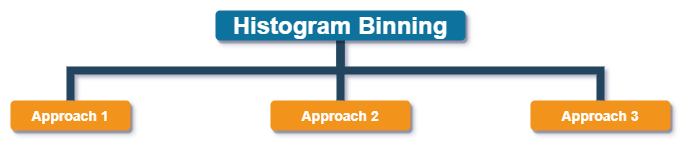
\includegraphics[scale= 0.5]{./Pictures/histogram_binning.png}
  \caption{Testing Module}
  \label{fig:Ch05F001}
\end{figure}




\subsection{Approach 1: Global Histogram using only magnitudes of optical flow}
In this section, we would discuss a global Histogram using only magnitudes of the optical flow of two consecutive images.
We are taking magnitudes part only of optical flow. Since our image size was \[120 \ast 160\], our input would be of size $19200$. We would sort the vector X into bins with intervals defined by the vector $numBins$ (Number of bins). Finally, it would output the frequency of elements in each bin. It would be returned as a feature row vector of size $9$.
The sample feature vector for two input images is the following:

\[[18611 ,173 ,142 ,115 ,71 ,50 ,29 ,4 ,5] \]



\subsection{Approach 2: Global Histogram using magnitudes and Orientation of optical flow}
In this section, we would discuss global histogram using magnitudes and Orientation of the optical flow of two consecutive images.

We are taking magnitudes and Orientation of optical flow. Since our image size was $120 \ast 160$, our input would be two matrices of size $120 \ast 160$.We would convert $120 \ast 160$ matrices to $19200$ vectors and calculation would be done.

It would create a Histogram of optical flow (HOOF) of the images, based on the respective weightage of magnitude with respect to orientations.
 Finally, it would output the frequency of elements in each bin. It would be returned as a feature row vector of size $9$.
 
 Sample feature vector for two input images is following:
\[[68.98, 5.93, 0, 0, 0, 0, 0, 0,21.13]\]





\subsection{Approach 3: Fractional Histogram Binning using  magnitudes and Orientation of optical flow taken over 8 x 8 cell}

In this section, we would discuss fractional Histogram using magnitudes and orientation of the optical flow of two consecutive images.
In this approach, we compute a HOOF descriptor vector for the supplied optical flow of two consecutive images.

We are taking magnitudes and orientation of optical flow. Since our image size was $120 \ast 160$, our input would be two matrices of size $120 \ast 160$. It would compute a local histogram of optical flow (HOOF) of $8 \ast 8$ pixel cells and concatenate to form a $9576$ feature vector.

The block size of $2 \ast 2$ cells is taken. There would be $9$ bins for each cell, \newline
so 
\[9 \ast 4 = 36\]
feature vector for a block. There would be a $50\%$ overlap between blocks. So that $15$ iterations over the vertical cell and $20$ repetitions over the horizontal cell.

\[{Feature\_Vector}_{\textbf{Total}} = (15 - 1) \ast (20 - 1 ) \ast 4 \ast 9 = 9576\]

It would be returned as a feature row vector of size 9.

 
 Sample feature vector of size $9576$ for two input images is following:
 
\[[0.004,0.002,0.543,0,0,...,0.003,0.006]\]
 
